% !TeX spellcheck = de
\documentclass[10pt,a4paper]{beamer}
%\documentclass[10pt,a4paper,handout]{beamer}

\usepackage[german]{babel} % deutsch und deutsche Rechtschreibung
\usepackage[utf8]{inputenc}
\usepackage[T1]{fontenc} % Umlaute und deutsches Trennen
\usepackage{amsmath}
\usepackage{amsfonts}
\usepackage{amssymb}
\usepackage{mathabx}
\usepackage{graphicx}
\usepackage{url}
\usepackage{color}
\usepackage{listings}
\usepackage{multicol}
\usepackage{xspace}
\usepackage[normalem]{ulem}
\usepackage{wasysym}

\DeclareGraphicsExtensions{.pdf,.jpeg,.png}
\graphicspath{{img/}}

% Klammern {{{
\newcommand{\lrk}{\left(}
\newcommand{\rrk}{\right)}
\newcommand{\lgk}{\left\{}
\newcommand{\rgk}{\right\}}
\newcommand{\lek}{\left[}
\newcommand{\rek}{\right]}
% }}}

\newcommand{\field}[1]{\ensuremath{\mathbb{#1}}\xspace}
\newcommand{\N}{\field{N}}
\newcommand{\Z}{\field{Z}}
\newcommand{\Q}{\field{Q}}
\newcommand{\R}{\field{R}}
\newcommand{\C}{\field{C}}
\newcommand{\K}{\field{K}}

\newcommand{\inda}[2]{\textit{Induktionsanfang ($#1=#2$): }}
\newcommand{\indv}{\textit{Induktionsvoraussetzung ($\star$): }}
\newcommand{\inds}[1]{\textit{Induktionsschritt ($#1\rightsquigarrow #1+1$): }}
\newcommand{\proofend}{\begin{flushright}$\Box$\end{flushright}}

\newcommand{\BigO}[1]{\ensuremath{\operatorname{O}\bigl(#1\bigr)}}

\newcommand{\ent}{\mathrel{\widehat{=}}}

%\newcommand{\hr}{\noindent\makebox[\linewidth]{\rule{\paperwidth}{0.4pt}}\vspace{0.6em}\\}
%\newcommand{\newslide}{}

\newcommand{\hr}{\noindent\makebox[\linewidth]{\rule{\paperwidth}{0.4pt}}\vspace{0.6em}\\\pause}
\newcommand{\newslide}{\pause}


\newenvironment{card}[1]
  {\begin{frame}[fragile,environment=card]#1}
  {\end{frame}}
  
\lstset{
  inputencoding=utf8,
  basicstyle=\footnotesize\ttfamily,
  tabsize=2,
  breaklines=true,
  prebreak=\mbox{$\ \curvearrowright$},
  keepspaces=true,
  %columns=flexible,
  keywordstyle=\bfseries\color{blue},
  stringstyle=\color{red!40!black},
  commentstyle=\itshape\color{green!40!black},
  identifierstyle=\color{blue!40!black}
}


%\pgfpagesuselayout{4 on 1}[a4paper,landscape,border shrink=5mm]
%\newcommand{\hr}{\noindent\makebox[\linewidth]{\rule{\paperwidth}{0.4pt}}\vspace{0.6em}\\}
%\newcommand{\newslide}{}

\newcommand{\hr}{\noindent\makebox[\linewidth]{\rule{\paperwidth}{0.4pt}}\vspace{0.6em}\\\pause}
\newcommand{\newslide}{\pause}


\begin{document}
\begin{card}
	\frametitle{Übung 1: Einführung}
	\url{http://people.f4.htw-berlin.de/~hebold/htw/pka/exercises/einf\%C3\%BChrung.pdf}
\end{card}

\begin{card}
	Gegeben: $f_1(x) = x^2-2$, $f_2(x) = x-5$, $f_3(x) = e^{x-2}$,  $f_4(x) = ln(x+5)$, $f_5(x) = 5$
	\vfill
	\begin{columns}
		\begin{column}{.5\linewidth}
		Bestimmen Sie die Ausdrücke der folgenden Funktionen:
			\begin{enumerate}[a)]
			\item $f_1 \circ f_2$
			\item $f_1 \circ f_2 \circ f_3$
			\item $(f_1 + f_4) \circ f_2$
			\item $f_3 \circ (f_1 + f_4) \circ f_2$
			\item $f_4 \circ f_4^{-1}$
			\item $ f_4^{-1} \circ f_4$
			\item $f_2 \circ f_3 \circ f_3^{-1} \circ f_2^{-1}$
			\item $f_1 \circ f_5 \circ f_5^{-1} \circ f_1^{-1}$
			\end{enumerate}
		\end{column}
		\begin{column}{.5\linewidth}
		\pause
		Lösung:
			\begin{enumerate}[a)]
			\item $(x-5)^2-2$
			\item $(e^{x-2}-5)^2-2$
			\item $(x-5)^2-2+ln(x)$
			\item $e^{(x-5)^2-2+ln(x)-2}$
			\item $id \text{ (da } f_4^{-1} \text{existiert)}$
			\item $id \text{ (da } f_4^{-1} \text{existiert)}$
			\item $id \text{ (da } f_2^{-1} \text{,} f_3^{-1} \text{existiert)}$
			\item \lightning ($f_5^{-1}$ existiert nicht)
			\end{enumerate}
		\end{column}
	\end{columns}
	\vfill
	Bilden Umkehrfunktion: $y = ln(x+5) \Leftrightarrow e^y = e^{ln(x+5)} \Leftrightarrow e^y = x+5 \Leftrightarrow e^y-5 = x \Rightarrow y = e^x-5$
\end{card}

\begin{card}
	Schreiben Sie in Java jeweils ein Programm, dass die Funktionen
	\begin{enumerate}[a)]
	\item $x+y$
	\item $x*y$
	\item $x^y$
	\end{enumerate}
	als int-Werten rekursiv berechnet
	\hr
	\begin{lstlisting}[language=Java]
public static int add(int x, int y) {
  if (y == 0) { return x; }
  return 1 + add(x, y-1);
}

public static int multiply(int x, int y) {
  if (y == 0) { return 0; }
  return x + multiply(x, y-1);
}

public static int pow(int x, int y) {
  if (y == 0) { return 1; }
  return x * pow(x, y-1);
}
	\end{lstlisting}
\end{card}

\begin{card}
	Schreiben Sie in Java Programme zu Berechnung der Fakultät mit dem Datentyp BigInteger rekursiv und iterativ.
	\hr
	$n! = 1 \cdot 2 \cdot ... \cdot (n-1) \cdot n = n  \cdot  (n-1)!$
	\begin{lstlisting}[language=Java]
	static int fac(int x) { return x == 0 ? 1 : x * fac(x-1); }
  BI = BigInteger
  static BI faci(BI x) {
    BI result = BI.ONE;
    for (BI i = BI.ONE; i.compareTo(x) <= 0; i = i.add(BI.ONE)) {
      result = result.multiply(i);
    }
    return result;
  }

  static BI facer(BI x) {
    if (x.compareTo(BI.ONE) <= 0) {
        return BI.ONE;
    }
    return x.multiply(facer(x.subtract(BI.ONE)));
  }
	\end{lstlisting}
\end{card}

\begin{card}
	Collatz-Problem Definition:\\
	$f: \mathbb{N} \rightarrow \mathbb{N}$ mit
	$f(1) = 1$, n gerade: $f(n) = n / 2$,n ungerade: $f(n) = 3n + 1$\\
	$F: \mathbb{N} \rightarrow \mathbb{N}$ mit $F(1) = f(1)  = 1$, $F(n) = F(f(n))$

	Collatz-Problem: Ist F für jedes $n \in \mathbb{N}$  definiert, d.h. $\forall n \in \mathbb{N}$ $\exists$ $F(n) \in \mathbb{N}$?
	\hr
	\begin{lstlisting}[language=Java]
static int f(int x) {
  if (x == 1) { return 1; }
  else if (x % 2 == 0) { return x / 2; }
  return 3 * x + 1;
}
static int F(int x) {
  if (x == 1) return 1;
  System.out.print("[" + x + "]");
  return F(f(x));
}
static int Flength(int x, int c) {
  if (x == 1) return c;
  return Flength(f(x), c + 1);
}
static int Flength(int x) {return Flength(x, 1);}
	\end{lstlisting}
\end{card}

\begin{card}
	Relationen, mit $R \subseteq M \times M$\\
	\begin{tabular}{ll}
		Reflexivität:& $(x, x) \in R $\\
		Symmetrie:&	$(x, y) \in R \Rightarrow (y, x) \in R$\\
		Antisymmetrie:& $(x, y) \in R, (y, x) \in R \Rightarrow x=y$\\
		Asymmetrie:& $(x, y) \in R \Rightarrow (y, x) \notin R$\\
		Transitivität:& $(x, y) \in R, (y, z) \in R \Rightarrow (x, z) \in R$\\
		Funktion: & bijektiv = surjektiv (rechtstotal, isOnto) +\\
	     	      & injektiv (linkseindeutig, isOneOne)
		\end{tabular}
		\begin{figure}[h]
		\centering
		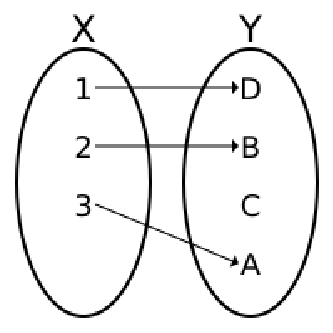
\includegraphics[width=3cm]{Injection.pdf}
		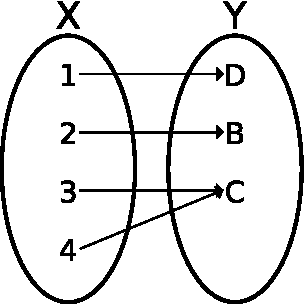
\includegraphics[width=3cm]{Surjection.pdf}
		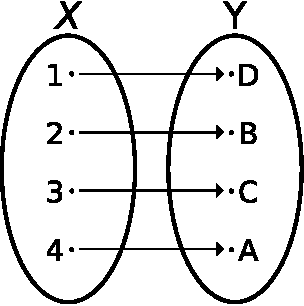
\includegraphics[width=3cm]{Bijection.pdf}
		\caption{injektive, surjektive, bijektive Abbildung}
		\end{figure}
\end{card}

\begin{card}
	Mengen: $A = \{3, 4\}$, $B = \{\{3, 4\}\}$\\Welche Behauptung stimmt?
	\begin{enumerate}[a)]
	\item $A = B$
	\item $A \subseteq B$
	\item $A \subsetneq B$
	\item $|A| = |B|$
	\end{enumerate}
	\hr
	\begin{enumerate}[a)]
	\item Nein, da unterschiedlich mächtig. siehe 4.)
	\item Nein, da gelten muss: $\forall x \in A: x \in B$, aber hier: $3,4 \notin B$
	\item A keine echte Teilmenge von B, da gelten muss: $A \subset B \land A \neq B \Rightarrow a.) \land \lnot b.)$ , a.) ist falsch
	\item Nein, da $2 \neq 1$
	\end{enumerate}
\end{card}

\begin{card}
	Das kartesische Produkt zweier Mengen A und B ist wie folgt definiert:
	$A \times B = \{(x,y):x	\in	A \land	y \in B\}$\\
	Prüfen Sie, ob das kartesische Produkt assoziativ ist, d.h. ob für Mengen X,Y,Z gilt:
	$(X	\times Y)\times Z=X \times(Y \times Z)$
	\hr
	Nein, da die Tupel $((x,y),z)$ und $(x,(y,z))$ unterschiedlich sind, also eine andere Struktur haben.
\end{card}

\begin{card}
	Welcher der folgenden Ausdrücke ist korrekt?
	\begin{enumerate}[a)]
	\item $0 \in \emptyset$
	\item $0 = \emptyset$
	\item $0 \subseteq \emptyset$
	\item $\{0\} \subseteq \emptyset$
	\end{enumerate}
	\hr
	\begin{enumerate}[a)]
	\item Nein, die leere Menge hat keine Elemente
	\item Nein, Zahlen sind keine Menge
	\item Nein, siehe b.)
	\item Nein, siehe a.)
	\end{enumerate}
\end{card}

\begin{card}
	Sei X eine Menge endlicher Größe und $2^X$ die Potenzmenge von $X$. Welches Ergebnis liefern:
	\begin{enumerate}[a)]
	\item $|2^X \cup X|$
	\item $|2^X| \cup |X|$
	\end{enumerate}
	\hr
	Beispiel: Potenzmenge  $X = \{ a,b \} \Rightarrow 2^X = \{ \emptyset, \{ a \}, \{ b \} , \{ a,b \} \}$
	\begin{enumerate}[a)]
	\item $2^X \cup X = \{ \emptyset, \{ a \}, \{ b \} , \{ a,b \}, a, b\} \Rightarrow
	|2^X \cup X| = 2^{|X|} + |X|$
	\item \lightning Vereinigung ist nur auf Mengen definiert und nicht auf Zahlen.
	\end{enumerate}
\end{card}

\begin{card}
	\frametitle{Übung 2: Konzepte Abstraktion}
	\url{http://people.f4.htw-berlin.de/~hebold/htw/pka/exercises/konzepte-Abstraktion.pdf}
\end{card}

\begin{card}
	Knappsack:\\
	Bildet von unterschiedlichen Summen eine Menge von n Summanden. (vgl. Merkle-Hellman Verfahren)\\
	Beispiel: Die Folge der Werte $( 3, 4, 5 )$ liefert die Summen $0, 3, 4, 5, 7, 8, 9, 12$.
	\hr
	Bilde Potenzmenge der Eingabe und addiere Elemente dieser einzelnen Mengen.\\
	Zum Beispiel: $2^{\{ 3, 4, 5 \}} = \{\emptyset, \{3\}, \{4\}, \{5\}, \{3,4\}, \{4,5\}, \{3,5\}, \{3,4,5\} \}$
\end{card}

\begin{card}
	Nennen Sie mindestens 3 Gründe für Abstraktion.
	\hr
	\begin{enumerate}[a)]
	\item \textbf{Wiederverwendbarkeit} von allgemeinen Problemlösungen
	\item \textbf{Klassifizieren} von Problemen, erkennen der Struktur
	\item Allgemeine Lösung zu detaillierten Problemen ($\approx$ \textbf{Kompression})
	\item \textbf{Ver\uline{ein}fachung}, reduzieren auf gemeinsame Eigenschaft
	\end{enumerate}
\end{card}

\begin{card}
	Inwiefern wird beim Programmieren ganz generell abstrahiert?
	\hr
	\begin{itemize}
	\item OOP (A) $\Leftrightarrow$ reale Welt (K)
	\item Programmcode (A) $\Leftrightarrow$ Problembeispiele (K)
	\item Programme (A)$\Leftrightarrow$ Prozesse / Programmlauf (K)\\(vgl. Debuggen - ständiger Kontextwechsel)
	\end{itemize}
	Legende: Konkretisierung (K), Abstraktion (A)
\end{card}

\begin{card}
	Inwiefern wird bei der \textbf{strukturierten} Programmierung abstrahiert?
	\hr
	if, for, while-Konstrukte ersetzen Sprungbefehle\\
	Beispiel: 
	\begin{lstlisting}[language=C]
	while(c > 0) {
	  c--;
	}
	\end{lstlisting}
	wird zu 
	\begin{lstlisting}[language=C]
	start:
	if(c <= 0) goto end;
	  c--;
	  goto start;
	
	end: ...
	\end{lstlisting}
\end{card}

\begin{card}
	Inwiefern wird bei der \textbf{prozeduralen} Programmierung abstrahiert?
	\hr
	\begin{itemize}
	\item parametrisierte Prozeduren ersetzen alle Werte-Kombinationen beim Aufruf\\
		Beispiel: f(x) $\ent$ f(1), f(2), ... f(n)
	\item Prozeduren ersetzen konkrete Implementierungen ($\approx$ \textbf{Blackbox})\\
		Beispiel: sort(array[] field) sortiert ohne, dass bekannt ist wie.
	\end{itemize}
\end{card}

\begin{card}
	Inwiefern wird bei der \textbf{modularen} Programmierung abstrahiert?
	\hr
	\begin{itemize}
	\item Kein konkreten Zustände, d.h. nur statische (vgl. \texttt{static}) Werte ($\approx$ \textbf{Zustandslos})
	\item Implementierung unbekannt, Referenzierung über Name ($\approx$ \textbf{Blackbox})\\
		Beispiel: \texttt{import java.io} $\rightarrow$ \texttt{import java.nio} bei gleicher API
	\end{itemize}
\end{card}

\begin{card}
	Inwiefern wird bei der \textbf{objekt-orientierten} Programmierung abstrahiert?
	\hr
	\begin{itemize}
	\item Vererbung, generischen Datentypen\\
			Beispiel: A extends B\\
			(A Konkretisierung  von B $\leftrightarrow$ B Generalisierung/Abstraktion von A)
	\item Polymorphismus, dynamisches Binden\\
		Beispiel:
		\begin{lstlisting}[language=Java]
		class B {
		  void f() { out.println("B"); }
		}
		
		class A extends B {
		  void f() { out.println("A"); }
		}
		
		B testA = new A();
		testA.f(); // "A"
		B testB = new B();
		testB.f(); // "B"
		\end{lstlisting}
	\end{itemize}
\end{card}

\begin{card}
	Inwiefern wird bei der \textbf{funktionalen} Programmierung abstrahiert?
	\hr
	\begin{itemize}
	\item Nur Funktionen und Rückgabewerte, keine Unterscheidung zwischen Daten(typen) und  Objekten\\
		Beispiel:
		%eigentlich JavaScript
		\begin{lstlisting}[language=Java] 
		function addiere(x,y) {
		  if (typeof y === "undefined" ) {
		    return function (y) { return x + y; }
		  }
		  return x + y;
		}
		addiere(2,4); // 6 
		var addiere_zu_drei = addiere(3)
		addiere_zu_drei(5) // 8
		\end{lstlisting}
		%Quelle: https://de.wikipedia.org/wiki/Currying#JavaScript
	\item Überladen von Funktionen\\
		Beispiel: \texttt{summe(a,b,c)} (A) und \texttt{summe(a,summe(b,c))} (K)
	\end{itemize}
\end{card}

\begin{card}
	Inwiefern wird bei der Programmierung abstrakter Datentypen abstrahiert?
	\hr
	\begin{itemize}
	\item Lists, Arrays als Abstraktion\\
		vgl. Gruppe (Math.), generische Datentypen\\
		Beispiele: 
		\begin{lstlisting}[language=Java] 
		static Object getFirst(ArrayList b) {
		   return ...
		}
		
		ArrayList a = new ArrayList<Integer>();
		...
		<?> c = getFirst(a);
		\end{lstlisting}
	\end{itemize}
\end{card}

\begin{card}
	Beim Abstraktionskonzept wird auf verschiedenen konkreten Objekten mit einem Namen referiert, wobei die Besonderheiten unberücksichtigt bleiben - von diesen wird abstrahiert.\\
	Bei der Konkretisierung wird umgekehrt einem Namen ein bestimmtes konkretes Objekt zugeordnet - der Name wird gebunden.\\
	Wann erfolgt im Rahmen der Programmierung die Konkretisierung, d.h. die Bindung	eines Namens?
	\hr
	Die Konkretisierung erfolgt zur \textbf{Laufzeit}, d.h. bei der Zuweisung wird der Typ und Name konkret festgelegt.\\
	Beispiel:
	\begin{lstlisting}[language=Java]
	// Abstraktion: Instanziierung
	List x = new ArrayList();
	// Konkretisierung: Zuweisung, Casting
	void doSth(List x) {ArrayList y=(ArrayList)x;}
	\end{lstlisting}
\end{card}

\begin{card}
	Imperative Programmierung:\\
	Von was wird durch einen Variablennamen abstrahiert?
	\hr
	Vom konkreten Wert hinter dem Variablennamen, da nur die Referenz auf den Wert benutzt wird.\\
		Beispiel: \texttt{int x = 3; x = 7;}
\end{card}

\begin{card}
	Imperative Programmierung:\\
	Von was wird durch Pointer abstrahiert?
	\hr
	Von der Speicheradresse\\
	Beispiel:
	\begin{lstlisting}[language=C]
	int *myPointer = 3 //Wert
	myPointer = 1234 // Speicheradresse
	\end{lstlisting}
\end{card}

\begin{card}
	Imperative Programmierung:\\
	Von was wird durch eine Initialisierung \texttt{int i=42} bzw. Zuweisung abstrahiert?
	\hr
	\begin{itemize}
	\item Speicherreservierung + Zuweisung und Belegung
	\item Darstellung
	\end{itemize}
	Beispiel: Big Endian / Little Endian (dt.: Byte-Reihenfolge)
\end{card}

\begin{card}
	Imperative Programmierung:\\
	Von was wird durch 
	\begin{itemize}
	\item if-Abfrage
	\item for-Schleife \texttt{for(int i=0;i<a;i++) block} 
	\item while-Schleife
	\end{itemize}
	abstrahiert?
	\hr
	if-, for- und while-Konstrukte ersetzen verschiedene Goto-Anweisungen und Labels 
	\begin{lstlisting}[language=C]
	while(c>0) {
	  c--;
	}
	\end{lstlisting}
	wird zu 
	\begin{lstlisting}[language=C]
	start:
	if(c <= 0) goto end;
	  c--;
	  goto start;
	
	end: ...
	\end{lstlisting}
\end{card}

\begin{card}
	Imperative Programmierung:\\
	Von was wird durch eine 
	\begin{enumerate}[a)]
	\item Prozedur (void)
	\item Funktion (non-void)
	\end{enumerate}
	abstrahiert?
	\hr
	\begin{enumerate}[a)]
	\item Implementierung
	\item Implementierung und Rückgabewert von der Funktion
	\end{enumerate}
\end{card}

\begin{card}
	Imperative Programmierung:\\
	Von was wird in C und C++ und Java durch den abstrakten Datentyp Array abstrahiert?
	\hr
	Von den Speicherbereichen, relativer Zugriff\\
	C und C++: Speicherbereiche sind zusammenhängend\\
	Beispiel: 
	\begin{lstlisting}
	int arr [] = {1,2,3};
	arr[0]
	\end{lstlisting}
	
	Java: Speicherbereiche sind nicht zwingend zusammenhängend\\
	Beispiel: 
	\begin{lstlisting}
	new int[]{1,2,3}[0]
	\end{lstlisting}
	
\end{card}

\begin{card}
	Imperative Programmierung:\\
	Funktionen werden in C, C++ und Java durch Aufrufe zur Laufzeit konkretisiert. Signatur und Methode sind die Abstraktionen. Zusätzlich bietet C++ Funktionen mit default Parametern. Was bedeuten diese für Abstraktion und Konkretisierung?
	\hr
	Default Parameter ermöglichen es, dass die überladene Methode nicht konkret die ursprüngliche Methode aufrufen muss. Es kann abstrakt die selbe Signatur mit den default Parametern verwendet werden.
\end{card}

\begin{card}
	Imperative Programmierung:\\
	Von was wird in C++ durch eine inline-Funktion abstrahiert?
	\hr
	Wie Makros als Textersetzung ohne Stack / Heap, jedoch wie Funktion mit Auswertung.
	Konkrete Ersetzung des Wertes ohne Aufbau Stack / Heap.
	\vfill
	Abgrenzung: Makro $\Leftrightarrow$ Inline-Funktion\\
	Haben beide keine Stack / Heap, d.h. beide arbeiten mit Textersetzung. Inline-Funktionen sehen aber aus wie Funktionen. 
	Problem bei Texterzersetzung mit Mehrfachaufruf, Beispiel: 
	\begin{lstlisting}
	Max(x,y) = {x > y ? x : y}
	Max(x++, y++)
	\end{lstlisting}
\end{card}

\begin{card}
	Objektorientierte Programmierung:\\
	Von was wird in Java durch eine Referenz \texttt{Type ref} abstrahiert?
	\hr
	\texttt{Type}: Für alle Objekt-Typen und deren Ableitung von Type\\
	\texttt{ref} steht für ein konkretes Objekt vom Typ \texttt{Type} oder einer Subklasse davon.
\end{card}

\begin{card}
	Objektorientierte Programmierung:\\
	Die meisten objektorientierter Sprachen verfügen über primitive Datentypen wie z.B. \texttt{int}. Warum haben diese primitiven Datentypen aus der Sicht des Abstraktionskonzepts einen Sonderstatus?
	\hr
	\begin{itemize}
	\item Call-by-Value: Passen direkt in Speicher ohne Referenzzugriff
	\item keine Kapselung notwendig/möglich
	\item Vererbung nicht möglich, da keine Klasse.
	\end{itemize}
\end{card}

\begin{card}
	Objektorientierte Programmierung:\\
	Was wird durch die ausschließliche Verwendung von Klassen, Objekten und Referenzen, d.h. durch die Streichung der primitiven Datentypen, im Sinne des Abstraktionskonzepts erreicht?
	\hr
	\begin{itemize}
	\item Kontinuität (Einheitlichkeit)
	\item Gemeinsamer Oberdatentyp, von dem alles erbt $\rightarrow$ ein einziger Vererbungsbaum
	\end{itemize}
\end{card}

\begin{card}
	Objektorientierte Programmierung:\\
	C++ und Java kennen die Möglichkeit des \textbf{overriding} (überschreiben). Inwiefern handelt es sich um eine Abstraktion? D.h. von welchen konkrete Elementen wird abstrahiert? 
	\hr
	Der Funktionsname ist die Abstraktion von der konkreten Implementierung der Objekt-Methode, da sich durch das überschreiben die Implementierung je nach Konkretisierung ändert.
\end{card}

\begin{card}
	Objektorientierte Programmierung:\\
	Mehrfachvererbung ist in Java bei Klassen nicht zugelassen. 
	\begin{enumerate}[a)]
	\item Nennen Sie eine Begründung im Rahmen des Abstraktionsprinzips.
	\item Wieso ist Mehrfachvererbung bei Interfaces zugelassen?
	\item Wie löst C++ die genannten Probleme?
	\end{enumerate}
	\hr
	\begin{enumerate}[a)]
	\item Overriding von Methoden ist durch die Einfachvererbung eindeutig
	\item Es steckt keine konkrete Implementierung dahinter
	\item Durch die Reihenfolge der Vererbung (erst beste Funktion wird genutzt)
	\end{enumerate}
\end{card}

\begin{card}
	Objektorientierte Programmierung:\\
	Inwiefern handelt es sich bei der Definition von Superclasses (Oberklassen) um eine Abstraktion?
	\hr
	\begin{itemize}
	\item Verallgemeinerung (Generalisierung / Abstraktion) der konkreten Klasse, mit allgemeineren und weniger Eigenschaften
	\item Allgemeingültige Oberklasse für alle Unterklassen
	\end{itemize}
\end{card}

\begin{card}
	Funktionale Programmierung:\\
	Inline-Funktionen sind Teil der meisten funktionalen Sprachen. Beschreiben Sie im Rahmen des Abstraktionskonzepts das Problem mit rekursiv definierten (inline-) Funktionen.
	\hr
	Eine rekursive Definition ist bei Inline-Funktionen (vgl. Makros) nicht möglich, da die Textersetzung unendlich ausgeführt wird.\\
	Beispiel:\\
	\begin{lstlisting}[language=C]
	inline int add(a, b) {
	  if(b == 0) return 1; // ignoriert,
	  return add(a, b-1) + 1; // da hier nur Textersetzung
	}
	\end{lstlisting}
	
\end{card}

\begin{card}
	Funktionale Programmierung:\\
	Inwiefern kann man sagen, dass in rein funktionalen Sprachen auf einer höheren Stufe der Abstraktion programmiert wird?
	\hr
	\begin{itemize}
	\item Alles ist eine Funktion: Werte, Klassen und das Programm selbst. Es gibt keine Unterscheidung
	\item Funktionen können (zur Laufzeit) erzeugt und verändert werden.
	
	\end{itemize}
	Beispiel: Lamda-Ausdrücke
\end{card}

\begin{card}
	Funktionale Programmierung:\\
	In rein funktionalen Sprachen sind Funktionen als Parameter und Rückgabewerte von Funktionen zugelassen. 
	\begin{enumerate}[a)]
	\item  Inwiefern wird dadurch eine höhere Stufe der Abstraktion erreicht, als Paradigmen bei Sprachen, die dieses Feature nicht haben?
	\item Ist es möglich, durch diese Erweiterung Probleme zu lösen, die in imperativen Sprachen nicht gelöst werden können?
	\end{enumerate}
	\hr
	\begin{enumerate}[a)]
	\item Abstraktion der Kontrollstruktur: dynamischer Kontrollfluss (Bsp: Callbacks), Funktionen können zur Laufzeit konstruiert/modifiziert werden.
	\item  Nein. wie bei imperativen Sprachen. Gegenbsp.: Ackermann ist imperativ nicht lösbar, sondern nur rekursiv. TODO: Frage
	\end{enumerate}
\end{card}

\begin{card}
	\frametitle{Übung 3: Paradigmen}
	\url{http://people.f4.htw-berlin.de/~hebold/htw/pka/exercises/konzepte-Paradigmen.pdf}
\end{card}

\begin{card}
	Das von-Neumann-Rechnerkonzept (auch von-Neumann-Architektur) zählt zur archetypischen Realisierung des imperativen Programmierparadigmas. Warum?
	\hr
	Imperative Konzept $\ent$ Befehlsorientiert\\
	Fetch, Execute-Zyklus
\end{card}

\begin{card}
	Die Turing-Maschine realisiert ebenfalls das imperativen Programmierparadigma. Warum?
	\hr
	Jeder Zustand verknüpft über Befehle, vgl. Überführungsfunktion
\end{card}

\begin{card}
	Wieso wird vom von-Neumann-Rechner\textbf{konzept} aber von der Turing-\textbf{Maschine} gesprochen?
	\hr
	Konzept: Abstraktion
	
	Maschine: Konkrete Idee (auch wenn so nicht realisierbar, durch das unendlich lange Band)
	\begin{figure}[h]
	\centering
	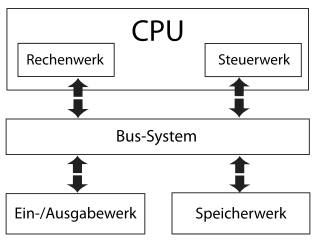
\includegraphics[width=4cm]{Von-Neumann_Architektur}
	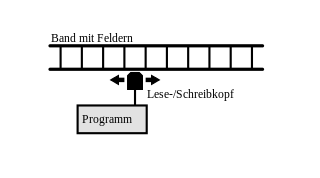
\includegraphics[width=6cm]{Turingmaschine}
	\caption{Von-Neumann, Turing-Maschine}
	\end{figure}
\end{card}

\begin{card}
	Im Zusammenhang mit dem Neumann-Rechnerkonzept ist die Rede vom von-Neumann-Flaschenhals, wenn Nachteile des Konzepts genannte werden.
	\begin{enumerate}[a)]
	\item Was ist darunter zu verstehen?
	\item Gibt es eine vergleichbare Problematik für die Turing-Maschine? 
	\end{enumerate}
	\hr
	\begin{enumerate}[a)]
	\item Alle Befehle / Daten müssen durch den Bus
	\item Schreib-/Lesekopf kann pro Zeiteinheit entweder schreiben oder lesen
	\end{enumerate} 
\end{card}

\begin{card}
	Nennen Sie wenigstens einen konzeptionellen Unterschied zwischen von-Neumann-Rechnerkonzept und Turing-Maschine.
	\hr
	Von TM ausgehend:
	
	\begin{itemize}
	\item Daten und Programme liegen \textbf{nicht} im selben Speicher
	\item keine Nummerierung/Adressierung eines Feldes auf dem Band
	\item keine Sprungadressen
	\item kann nur 1 Feld gehen pro Befehl
	\end{itemize}
\end{card}

\begin{card}
	Setzt die Turing-Maschine das von-Neumann-Rechnerkonzept um?
	\hr
	\textbf{Nein}, weil
	\begin{itemize}
	\item Bei TM: Daten $\neq$ Programme
	\item TM hat keine Sprungadresse
	\end{itemize}
	\vfill
	oder \textbf{Ja} mit Einschränkungen (vgl. Nein)
	\begin{itemize}
	\item Arbeiten befehlsorientiert
	\item Arbeiten deterministisch
	\end{itemize}
\end{card}

\begin{card}
	Wie könnte das Paradigma der strukturierten Programmierung in das von-Neumann-Rechnerkonzept integriert werden?
	\hr
	Überwachen bzw. Regeln der Sprunganweisungen.\\
	D.h. begrenzter Bereich (Scope) z.B. bei if-Anweisungen
\end{card}

\begin{card}
	Wieso verletzt das Konzept der lokalen static-Variablen in C das Paradigma der funktionalen
	Programmierung?
	\hr
	Funktionsausgabe nur abhängig von Eingabe. D.h. bei gleicher Eingabe gleiche Ausgabe (Idempotent, Deterministisch).
	\begin{lstlisting}[language=C]
	int f(int i) {
	  // Ausfuehrung bei Objekt-Init, 
	  // nicht bei Methodenaufruf
	  static int x = 0; 
	  x++;
	  return x+i;
	}
	\end{lstlisting}	
\end{card}

\begin{card}
	Wieso verletzen Pointer in C das Paradigma der funktionalen Programmierung?
	\hr
	Pardigma der f. Programmierung: Funktionsausgabe nur abhängig von Eingabe.  D.h. bei gleicher Eingabe gleiche Ausgabe.
	\begin{lstlisting}[language=C]
	int f(int *i) {
	  // Veraendern der Speicheradresse und 
	  //somit der Eingabe
	  *i = 1234;
	  ...
	}
	\end{lstlisting}	
\end{card}

\begin{card}
	In Java gibt es mit dem Collection-Framework eine Reihe von sogenannten Container-Klassen. Welches objektorientierte Programmierparadigma verletzen Objekte z.B. der Klassen	ArrayList oder Vector? 
	\hr
	Es werden Referenzen gespeichert. D.h. die Datenkapselung ist verletzt. Werte müssten unveränderlich (immutable) sein.
	\begin{lstlisting}[language=Java]
	class Dummy{int value;}
	...
	Dummy example = new Dummy()
	ArrayList<Dummy> list = new ArrayList<Dummy>()
	list.add(example);
	
	// Zugriff auf value ueber 2 Wege:
	example.value = 1;
	list.get(0).value = 2;
	\end{lstlisting}	
\end{card}

\begin{card}
	Wie müsste das Funktionskonzept in C beschränkt bzw. erweitert werden, damit es nicht zu Verletzungen des Paradigmas der funktionalen Programmierung kommen kann?
	\hr
	Zustandslosigkeit durch:
	\begin{itemize}
	\item kein static und Pointer 
	\item keine Systemaufrufe
	\end{itemize}
\end{card}

\begin{card}
	Das funktionale Programmierparadigma, das die referentielle Transparenz der Variablen fordert, wird in C durch die Zuweisung verletzt. 
	\begin{enumerate}[a)]
	\item Wie müssten die Regeln für die Verwendung der Zuweisung geändert werden, damit die	Zuweisung in das funktionale Konzept passt?
	\item Welcher Art von Anweisung entspräche die veränderte Zuweisung dann?
	\end{enumerate}
	\hr
	\begin{enumerate}[a)]
	\item Unveränderliche Variablen, Einmal-Zuweisung, bzw. nur Init.
	\item Konstanteninitialisierung
	\end{enumerate}
	
\end{card}

\begin{card}
	Die referentielle Transparenz sorgt dafür, dass Programme in rein funktionalen Sprachen	problemlos nebenläufig abgearbeitet werden können. 
	\begin{enumerate}[a)]
	\item Erklären Sie den Zusammenhang an einem Beispiel. 
	\item Erklären Sie an einem Beispiel den Zusammenhang fehlender referentieller Transparenz und Problemen bei nebenläufig ausgeführten Programmen. 
	\end{enumerate}
	\hr
	\begin{enumerate}[a)]
	\item Werte unveränderlich (immutable), d.h. kein Zustand und stark begrenzter Gültigkeitsbereich. Funktionen sind Thread-Safe, da Parameter nicht von außen geändert werden können.\\
	Beispiel: Immutable-Klassen sind automatisch thread-Safe, parallelisierbar und skalierbar. 
	\item Objekt-Parameter können während Thread-Unterbrechung über eine Referenz außerhalb der eigentlich Funktion verändert werden und haben somit einen anderen Zustand. Kein Determinismus, Race-Condition möglich.
	\end{enumerate}
\end{card}

\begin{card}
	Objektorientierte Sprachen kennen sogenannte inline-Funktionen.
	\begin{enumerate}[a)]
	\item Wieso sind inline-Funktionen in objektorientierten Programmiersprachen implementiert?
	\item Sind inline-Funktionen in rein funktionalen Programmiersprachen sinnvoll?
	\item Welches Problem ergibt sich aus inline-Funktionen im Rahmen einer rein funktionalen Sprache?
	\end{enumerate}
	\hr
	\begin{enumerate}[a)]
	\item Performancevorteile, da weniger Overhead ohne Heap / Stack.
	\item Ja, erhöhen Geschwindigkeit
	\item Rekursionen können nicht aufgelöst werden. Daher nur als Zusatz, nicht als Ersatz für normale Funktionen.
	\end{enumerate}
\end{card}

\begin{card}
	Angenommen in C würden innerhalb von parametrisierten Makros Zuweisungen nicht mehr	zugelassen sein.\\
	Inwiefern verletzen Makros dann trotzdem weiterhin Paradigmen der funktionalen Programmierung?
	\hr
	Variablen sind außerhalb vom Makro gültig, d.h vor oder nach dem Aufruf / Ersetzung.\\
	Durch die Textersetzung können Variablen(namen) genutzt werden, die erst im nachfolgenden Programm definiert werden. Dadurch ist Idempotenz / Determinismus verletzt.\\
	Beispiel:
	\begin{lstlisting}[language=C]
	#define printX print x
	int x = 100;
	printX(); // Ausgabe: 100
	\end{lstlisting}
\end{card}
\begin{card}
	\frametitle{Übung 4: Primitiv rekursive Funktionen}
	\url{http://people.f4.htw-berlin.de/~hebold/htw/pka/exercises/algorithmen-rekursiveFunktionen.pdf}
\end{card}

\begin{card}
  Formulieren Sie die folgenden Ausdrücke mit Hilfe von F = ${+, \cdot}$ und ${N, O, P^m_i, S^{n+1}, R}$:
	\begin{enumerate}[a)]
    \item[a)] $a \cdot b + c$
    \item[d)] $4 \cdot (3 + x)$
    \item[e)] $(a + b) \cdot (a + b)$
    \item[h)] $(a + b) \cdot (c + d)$
	\end{enumerate}
	\hr
	\begin{enumerate}[a)]
    \item[a)] $S(+, S(\cdot, P^3_1, P^3_2), P^3_3)(a, b, c)$
    \item[d)] $S(\cdot, P^3_1, S(+, P^3_2, P^3_3))(4, 3, x)$
    \item[e)] $S(\cdot, +, +)(a, b)$
    \item[h)] $S(\cdot, S(+, P^4_1, P^4_2), S(+, P^4_3, P^4_4))(a, b, c, d)$
	\end{enumerate}
\end{card}

\begin{card}
  Formulieren Sie eine primitiv rekursive Funktion, die
  \begin{enumerate}[a)]
    \item die arithmetische Differenz bestimmt.
    \item die das Vorzeichen prüft und 0 bei 0 und 1 bei Werten > 0 liefert.
    \item das Maximum von zwei Zahlen liefert.
	\end{enumerate}
	\hr
  \begin{enumerate}[a)]
    \item
      \begin{align*}
        pre &= S(R(O, P^3_2), P^1_1, O) \\
        \dotdiv &= S(R(P^1_1, pre \circ P^3_1)), P^2_2, P^2_1)(a, b)
      \end{align*}
    \item $sign = S(R(O, N \circ O \circ P^3_2), P^1_1, O)$
    \item
      \begin{align*}
        first &= S(\cdot, S(gt, P^2_1, P^2_2), P^2_1) \\
        sec &= S(\cdot, S(gt, P^2_2, P^2_1), P^2_2) \\
        eq' &= S(\cdot, S(eq, P^2_1, P^2_2), P^2_1) \\
        max &= S(add, S(add, first, sec), eq')
      \end{align*}
	\end{enumerate}
\end{card}

\begin{card}
  Formulieren Sie eine primitiv rekursive Funktion, die
  \begin{enumerate}
    \item[d)] den ganzzahligen Rest der Werte x und y bestimmt.
    \item[e)] die Teilbarkeit einer Zahl x hinsichtlich y prüft.
    \item[f)] die Operatoren $>, \geq, =$
    \item[g)] die absolute Differenz $|a - b|$
	\end{enumerate}
	\hr
  \begin{enumerate}
    \item[d)]
      \begin{align*}
        mod(a, b) &= a \dotdiv (a \text{ div } b) \cdot b \\
        div(a, b) &= \sum\limits_{i=1}^a \lrk \text{sign} \lrk \prod\limits_{j=1}^i a \dotdiv j \cdot b \rrk \rrk
      \end{align*}
    \item[e)] nsign($a$ mod $b$)
    \item[f)] $gt = sign(x \dotdiv y)$ \\
              $eq = nsign(gt(x, y) + gt(y,x))$ \\
              $ge = gt + eq$
    \item[g)] $absDiff(a,b) = diff(a, b) + diff(b, a) \\
	\end{enumerate}
\end{card}

\begin{card}
  0 und N sind Funktionen $\N \rightarrow \N, P, S^{n+1}$ und R dagegen
  Funktionen auf Funktionen, d.h. Operatoren. $S^{n+1}$ ist wie folgt definiert:
  \[
    (f, g_1,..., g_n) \mapsto a \in \N = S^{n+1}(f, g_1,..., g_n)
  \]

  \begin{enumerate}[a)]
    \item Wieso kann man sagen, dass $S^{n+1}$ für mehrere Operatoren steht?
    \item Wieviele verschiedene Operatoren ergeben sich aus $S^{n+1}$?
    \item Was bedeutet es für die Programmierung, dass es mehrere Operatoren $S^{n+1} $ gibt?
  \end{enumerate}
  \hr
  \begin{enumerate}[a)]
    \item Die $n$ $g$'s werden jeweils aufgerufen und bilden damit ein Funktionsschema.
    \item $n$
    \item Overloading muss möglich sein für unterschiedliche Stelligkeiten $n$
  \end{enumerate}
\end{card}

\begin{card}
  Der Ausdruck $S^{n+1}(f, g_1, \ldots, g_n)$ abstrahiert von der Anzahl $n$ möglicher Funktionen und der Stelligkeit von $f$.
  \begin{enumerate}[a)]
    \item Begründen Sie:
    \begin{enumerate}[i)]
      \item Es handelt sich also eigentlich um $n$ verschiedene Operatoren.
      \item Die Stelligkeit von $f$ ist $n$.
      \item Die Stelligkeit der Funktionen $g_1, \ldots, g_n$ ist $m$.
    \end{enumerate}
    \item Was bedeuten i) – iii) für die Implementierung (Programmierung) von $S^{n+1}$?
  \end{enumerate}
  \hr
  \begin{enumerate}[a)]
    \item Definition: $S^{n+1}(f, g_1, \ldots, g_n)(x_1, \ldots, x_m) = f(g_1(x_i, \ldots, x_m), \ldots, g_n(x_i, \ldots, x_m))$
    \begin{enumerate}[i)]
      \item Ja, da $g_i$ $n$-mal aufgerufen wird.
      \item Ja, da die Parameter $g_1, \ldots, g_n$ sind.
      \item Ja, da die Parameter von $g_i$ $x_1, \ldots, x_m$ ist.
    \end{enumerate}
    \item
    \begin{enumerate}[i)]
      \item Overloading / Variable Parameterliste muss in der Sprache vorhanden sein und benutzt werden oder $n$ unterschiedliche Funktionen müssen definiert werden.
      \item Overloading / Variable Parameterliste muss in der Sprache vorhanden sein und benutzt werden oder $n$ unterschiedliche Funktionen müssen definiert werden.
      \item Overloading / Variable Parameterliste muss in der Sprache vorhanden sein und benutzt werden oder $m$ unterschiedliche Funktionen müssen definiert werden.
    \end{enumerate}
  \end{enumerate}
\end{card}

\begin{card}
  Die Stelligkeit $m$ der Funktionen $g_1, \ldots, g_n$ spielt für den Operator $S^{n+1}(f, g_1, \ldots, g_n)$ im Rahmen des Konzepts der rekursiven Funktionen und bei den Fragestellungen der Berechenbarkeit keine Rolle.
  \begin{enumerate}[a)]
    \item Was ist mit dieser Aussage gemeint?
    \item Was bedeutet das für die Programmierung von $S^{n+1}$ ?
  \end{enumerate}
  \hr
  \begin{enumerate}[a)]
    \item $S$ ist nur für das Zusammenbauen der Funktionen $f$ mit den $g_i$'s zuständig. Daher ist $x_1, ..., x_m$
      unwesentlich.
    \item Die Funktion $S$ muss unabhängig von allen $g_i$ und $f$ funktionieren.
  \end{enumerate}
\end{card}

\begin{card}
  Die Stelligkeit $n$ der Funktion $f$ spielt für den Operator $S^{n+1}(f, g_1, \ldots, g_n)$ im Rahmen des Konzepts der rekursiven Funktionen und bei den Fragestellungen der Berechenbarkeit keine Rolle.
  \begin{enumerate}[a)]
    \item Was ist mit dieser Aussage gemeint?
    \item Was bedeutet das für die Programmierung von $S^{n+1}$ ?
  \end{enumerate}
  \hr
  \begin{enumerate}[a)]
    \item $f$ muss $n$ Funktionen akzeptieren können. $S^{n+1}$ ist das ganze egal.
    \item Die Funktion $g$ hat eine variable Parameterliste und daher muss Currying in der Sprache möglich sein.
  \end{enumerate}
\end{card}

\begin{card}
  Die Mehrstelligkeit der rekursiven Funktionen führt nicht aus der Menge der rekursiven Funktionen hinaus. Es spielt also keine Rolle, ob man $S, R$ und $\mu$ auf n-stellige oder ein-stellige Funktionen anwendet. Mit anderen Worten: Alle n-stelligen rekursiven Funktionen können durch einstellige rekursive Funktionen dargestellt werden.
  \begin{enumerate}[a)]
    \item Beschreiben Sie die Umsetzung.
  \end{enumerate}
  \hr
  \begin{enumerate}[a)]
    \item Durch das Currying wird eine mehrstellige Funktion $f(x_1, x_2)$ in mehrere einstellige Funktionen, die
      hintereinander ausgeführt werden, umgeformt: $f(x_1)(x_2)$
  \end{enumerate}
\end{card}

\begin{card}
Sie wollen eine primitiv rekursive Funktion definieren, die die Funktion
\[
f(x) =
\begin{cases}
1 & \text{wenn $x = 1$} \\
  \frac{x}{2} & \text{wenn $x$ gerade} \\
3 \cdot x + 1 &\text{wenn $x$ ungerade}
\end{cases}
\]
berechnet, d.h. die Formulierung erfolgt ausschließlich mit den Funktionen bzw. Funktionssymbolen $N, 0, P^m_i , S, R$.
  \begin{enumerate}[a)]
    \item Warum scheitern Sie?
  \end{enumerate}
  \hr
  \begin{enumerate}[a)]
    \item Da die Rekursion durch $R$ umgesetzt wird, muss $m$ gesetzt sein, sodass eine Schleife definiert wird. Bei der Ackermann-Funktion ist unklar, wie viele Durchläufe getätigt werden müssen, um das Ergebnis zu erhalten. Daher ist eine Endlos-Schleife notwendig und primitiv rekursive Funktionen können dies nicht umsetzen.
  \end{enumerate}
\end{card}

\begin{card}
  Was bedeutet die Aussage: „Alle berechenbaren Funktionen können mit Hilfe der Funktionen $0, N, P^m_i, S^{n+1}, R$ und $\mu$ formuliert werden“ für die Programmierung?
  \hr
  Die Ackermannfunktion ist umsetzbar und Endlosschleifen sind möglich. Alle berechenbare Probleme können mit primitiv rekursiven Funktionen umgesetzt werden.
\end{card}

\begin{card}
  Was unterscheidet die folgenden Aufzählfunktionen $\N^2 \rightarrow \N$ (Paare natürlicher Zahlen auf natürliche Zahlen) voneinander:
  \begin{itemize}
    \item $c(x, y) = \frac{(x + y)(x + y + 1)}{2}$
    \item $p(x, y) = 2^x \cdot 3^y$
  \end{itemize}
  \hr
  $c$ ist surjektiv. $p$ könnte bijektiv sein.
\end{card}

\begin{card}
	\frametitle{Übung 5: Induktion}
	\url{http://people.f4.htw-berlin.de/~hebold/htw/pka/exercises/algorithmen-Induktion.pdf}
\end{card}

\begin{card}
  Beweisen Sie mit Hilfe der vollständigen Induktion:\\
  $\forall n (n \in \N_0 \rightarrow 2^0 + 2^1 + \ldots + 2^n = 2^{n+1} - 1)$
  \hr
  \begin{align*}
    \forall n (n \in \N_0 \rightarrow 2^0 + 2^1 + \ldots + 2^n &= 2^{n+1} - 1) \\
    \sum\limits_{i=0}^n 2^i &= 2^{n+1} - 1 \\
    2^0 = 2^1 - 1 &= 1 & (IA: n=0) \\
    \sum\limits_{i=0}^{n+1} 2^i &= 2^{(n+1)+1} - 1 & (IS: n=n+1) \\
    \sum\limits_{i=0}^{n} 2^i + 2^{n+1} = 2^{n+2} - 1 \\
    2^{n+1} - 1 + 2^{n+1} &= 2^{n+2} - 1 & |+1 \\
    2^{n+1} + 2^{n+1} &= 2^{n+2} \\
    2 \cdot 2^{n+1} &= 2^{n+2} \\
    2^{n+2} &= 2^{n+2}
  \end{align*}
\end{card}

\begin{card}
  Beweisen Sie mit Hilfe der vollständigen Induktion:\\
  $n \in \N_0 \Rightarrow n^2 + n$ ist gerade
  \hr
  \begin{align*}
    \forall n (n \in \N_0 \rightarrow n^2 + n \text{ ist gerade}) \\
    0^2 + 0 \text{ ist gerade} \quad (IA: n=0) \\
    (n+1)^2 + (n+1) \quad (IS: n=n+1) \\
    n^2 + 2n + 1 + (n+1) \\
    n^2 + n \quad + \quad 2n + 2 \\
    n^2 + n \text{ ist gerade} \\
    2n + 2 \text{ ist gerade} \\
    \text{gerade } + \text{ gerade} = \text{ gerade} \\
  \end{align*}
\end{card}

\begin{card}
  Beweisen Sie mit Hilfe der vollständigen Induktion:\\
  $n \in \N_0 \Rightarrow 5^n + 7$ ist durch 4 teilbar
  \hr
  % TODO
  \begin{align*}
    4 &\mid 5^n + 7 \\
    4 &\mid (5^0 + 7 = 1+7 = 8) & (IA: n=0) \\
    4 &\mid (5^{n+1} + 7) & (IS: n=n+1) \\
    4 &\mid (5 \cdot 5^n + 7) & \\
    4 &\mid (5 \cdot 5^n + 7) & \\
    ...
  \end{align*}
\end{card}

\begin{card}
  Beweisen Sie mit Hilfe der vollständigen Induktion:\\
  $n \in \N_0 \Rightarrow 1 + 3 + 5 + \ldots + (2n - 1) = n^2$
  \hr
  \begin{align*}
    1 + 3 + 5 + \ldots + (2n - 1) &= n^2 \\
    \sum\limits_{i=1}^n 2i - 1 &= n^2 \\
    2 \cdot 1 - 1 &= 1^2 = 1 & (IA: n=1) \\
    \sum\limits_{i=1}^{n+1} 2i - 1 &= (n+1)^2 & (IS: n=n+1) \\
    \sum\limits_{i=1}^{n} 2i - 1 + 2 \cdot (n+1) - 1 &= (n+1)^2 & \\
    n^2 + 2 \cdot (n+1) - 1 &= (n+1)^2 & \\
    n^2 + 2n + 2 - 1 &= (n+1)^2 & \\
    n^2 + 2n + 1 &= (n+1)^2 & \\
    n^2 + 2n + 1 &= n^2 + 2n + 1
  \end{align*}
\end{card}

\begin{card}
  Beweisen Sie mit Hilfe der vollständigen Induktion:\\
  $n \in \N_0 \Rightarrow 3 \mid n^3 - n$
  \hr
  \begin{align*}
    3 \mid n^3 - n & \\
    3 \mid 0 - 0 & (IA: n=0) \\
    3 \mid (n+1)^3 - n & (IS: n=n+1) \\
    3 \mid n^3 + 3n^2 + 3n + 1 - (n+1) & \\
    3 \mid n^3 + 3n^2 + 3n + 1 - n - 1 & \\
    3 \mid n^3 - n \quad + \quad 3n^2 + 3n & \\
    3 \mid n^3 - n & \\
    3 \mid 3(k^2 + n) & \\
  \end{align*}
\end{card}

\begin{card}
  Beweisen Sie mit Hilfe der vollständigen Induktion:\\
  $n \in \N_0 \Rightarrow 0 \cdot 0! + 1 \cdot 1! + 2 \cdot 2! + \ldots + n \cdot n! = (n+1)!-1$
  \hr
  \begin{align*}
    0 \cdot 0! + 1 \cdot 1! + 2 \cdot 2! + \ldots + n \cdot n! &= (n+1)!-1 & \\
    \sum\limits_{i=0}^{n} i \cdot i! &= (n+1)!-1 & \\
    0 \cdot 0! &= (0+1)!-1 = 0 & (IA: n=0) \\
    \sum\limits_{i=0}^{n+1} i \cdot i! &= ((n+1)+1)!-1 & (IS: n=n+1) \\
    \sum\limits_{i=0}^{n} i \cdot i! + (n+1) \cdot (n+1)! &= (n+2)!-1 & \\
    (n+1)! - 1 + (n+1) \cdot (n+1)! &= (n+2)!-1 & \\
    n! \cdot (n+1) - 1 + (n+1) \cdot n! \cdot (n+1) &= (n+2)!-1 & \\
    n! - 1 + n!(n+1) &= (n+2)!-1 & \\
    n!(-1 + (n+1)) &= (n+2)!-1 & \\
    n!(n+2) &= (n+2)!-1 & ?? \\
  \end{align*}
\end{card}

\begin{card}
  Der reguläre Ausdruck \texttt{(10){n}} steht für eine Folge von binären Ziffern. Zeigen Sie, dass der Ausdruck für alle
  $n \geq 1$ dem Wert $\frac{2(4^n - 1)}{3}$ entspricht.
  \hr
  \begin{align*}
    \sum\limits_{i=1}^{n} 2^{2i-1} &= \frac{2(4^n - 1)}{3} & \\
    2 \cdot 1 - 1 &= \frac{2(4^1 - 1)}{3} = 1 & (IA: n=0) \\
    \sum\limits_{i=1}^{n+1} 2^{2i-1} &= \frac{2(4^{(n+1)} - 1)}{3} & (IS: n=n+1) \\
    \sum\limits_{i=1}^{n} 2^{2i-1} + 2^{2(n+1) - 1} &= \frac{2(4^{(n+1)} - 1)}{3} & \\
    \frac{2(4^{n} - 1)}{3} + 2^{2n+1} &= \frac{2(4^{(n+1)} - 1)}{3} & \\
    \frac{2(4^{n} - 1)}{3} + \frac{3 \cdot 2^{2n+1}}{3} &= \frac{2(4^{(n+1)} - 1)}{3} & |\cdot 3 \\
    2(4^{n} - 1) + 3 \cdot 2^{2n+1} &= 2(4^{(n+1)} - 1) & (nächste Folie) \\
  \end{align*}
\end{card}

\begin{card}
  Der reguläre Ausdruck \texttt{(10){n}} steht für eine Folge von binären Ziffern. Zeigen Sie, dass der Ausdruck für alle
  $n \geq 1$ dem Wert $\frac{2(4^n - 1)}{3}$ entspricht.
  \hr
  \begin{align*}
    2(4^{n} - 1) + 3 \cdot 2^{2n+1} &= 2(4^{(n+1)} - 1) & |:2 \\
    4^{n} - 1 + 3 \cdot 2^{2n} &= 4^{(n+1)} - 1 & |+1 \\
    4^{n} + 3 \cdot 2^{2n} &= 4^{(n+1)} & \\
    4^{n} + 3 \cdot 4^n &= 4^{(n+1)} & \\
    4^{n} + 3 \cdot 4^n &= 4^{(n+1)} & \\
    (1+3) \cdot 4^{n} &= 4^{(n+1)} & \\
    4 \cdot 4^{n} &= 4^{(n+1)} & \\
    4^{n+1} &= 4^{(n+1)} & \\
  \end{align*}
\end{card}

\begin{card}
  Jemand stellt die Behauptung auf $\forall n : n \in \N \rightarrow \varphi(n)$ mit $\varphi(n) = (n+2 = n+1)$ und beweist sie unter Hinweis auf $\varphi(n) \Rightarrow \varphi(n^+)$.
  \begin{enumerate}[a)]
    \item Zeigen Sie, dass der Induktionsschritt gültig ist.
    \item Zeigen Sie, dass die Verallgemeinerung, also der Induktionsschluss falsch ist.
  \end{enumerate}
  \hr
  TODO
\end{card}

\begin{card}
  Zeigen Sie mit Hilfe der vollständigen Induktion, dass die Anzahl der Elemente der Potenzmenge $P(A)$ einer endlichen
  Menge $A$ gleich $2^{|A|}$ ist.
  \hr
  TODO
\end{card}

\begin{card}
  Einer der Grundsätze der Zahlentheorie besagt, dass alle natürlichen Zahlen in Faktoren aus Primzahlen zerlegt werden
  können: $m = p_1^{e_1} \cdot \ldots \cdot p_n^{e_n}$. Beweisen Sie den Grundsatz mit Hilfe der Wertverlaufsinduktion.
  \hr
  TODO
\end{card}

\begin{card}
  In der Analysis gilt die folgende verallgemeinerte Produktregel:
  \[
  (f_1 \cdot f_2 \cdot \ldots \cdot f_n)' = (f_1' \cdot f_2 \cdot \ldots \cdot f_n) + (f_1 \cdot f_2' \cdot \ldots \cdot f_n) + \cdot + (f_1 \cdot f_2 \cdot \ldots \cdot f_n')
  \]
  für die differenzierbare Funktionen $f_i$. Beweisen Sie den Satz mit Hilfe der Wertverlaufsinduktion.
  \hr
  \begin{align*}
    \lrk f_1 \rrk ' &= f_1' \\
    (f_1 \cdot f_2 \cdot \ldots \cdot f_{n+1})' &= (f_1' \cdot \ldots \cdot f_{n+1}) + \ldots + (f_1 \cdot \ldots \cdot f_{n+1}') \\
    &= ((f_1 \cdot f_2 \cdot \ldots \cdot f_n)(f_{n+1}))' \\
    &= (f_1 \cdot f_2 \cdot \ldots \cdot f_n)' \cdot f_{n+1} + (f_1 \cdot f_2 \cdot \ldots \cdot f_n) \cdot (f_{n+1})' \\
    &= f_1' \cdot f_2 \cdot \ldots \cdot f_n \cdot f_{n+1} + \ldots \\
    & \hspace{3.3cm} + f_1 \cdot f_2 \cdot \ldots \cdot f_n' \cdot f_{n+1} \\
    & \hspace{3.3cm} + f_1 \cdot f_2 \cdot \ldots \cdot f_n \cdot f_{n+1}' \\
    &= (f_1 \cdot f_2 \cdot \ldots \cdot f_{n+1})' \\
  \end{align*}
\end{card}

\begin{card}
	Die strukturelle Induktion setzt sich die Idee der vollständigen Induktion auf Mengen um. Wie lautet entsprechend:
  \begin{enumerate}[a)]
	  \item die Verankerung
	  \item der Induktionsschritt
	  \item die Verallgemeinerung
	\end{enumerate}
	bei der strukturellen Induktion?
	\hr
	\begin{enumerate}
	  \item Beweisen für die Grundelemente
	  \item Zeigen, dass sich grüßere Elemente rekursiv aus kleineren Elementen zusammensetzen.
	  \item Ist es für die Grundelemente und den Induktionsschritt bewiesen, so gilt die Verallgemeinerung.
	\end{enumerate}
\end{card}

\begin{card}
  Die Folge der Fibonacci-Zahlen ist für $n \in \N \, (\geq 1)$ wie folgt definiert ($m := n+2$):
  \[
    a_{m+2} =
\begin{cases}
  a_{m+1} + a_{m} & \qquad m > 0 \\
  1 & \qquad \text{sonst}
\end{cases}
  \]
  Beweisen Sie mit Hilfe struktureller Induktion für ($a_n$) die Gültigkeit folgender Sätze:
  \begin{enumerate}[a)]
    \item $1 + a_1 + a_2 + \ldots + a_n = a_{n+2}$
    \item $3 \mid n \Rightarrow a_{n}$ ist gerade und $3 \nmid n \Rightarrow a_{n}$ ist ungerade
	\end{enumerate}
	\hr
  \begin{enumerate}[a)]
	  \item
	    \begin{align*}
        n = 1: 1+a_1 &= a_{1+2} \\
        2 &= 2 \\
        n = 2: 1+a_1+a_2 &= a_{2+2} \\
        3 &= 3 \\
        1 + a_1 + \ldots + a_n + a_{n+1} &= a_{(n+1)+2} \\
        a_{n+2} + a_{n+1} &= a_{n+3} \\
	    \end{align*}
	  \item TODO
	\end{enumerate}
\end{card}

\begin{card}
  Zeigen Sie mit Hilfe der doppelten Induktion, dass xor für boolsche Ausdrücke nicht universell ist. (Hinweis: Die
  Tautologie ist nicht dargestellbar.)
	\hr
  \begin{tabular}{cc|c|c|c|c|c}
    a & b & $\oplus$ & $\land$ & $\lor$ & $\top$ & $\bot$ \\ \hline
    0 & 0 & 0 & 0 & 0 & 1 & 0 \\
    0 & 1 & 1 & 0 & 1 & 1 & 0 \\
    1 & 0 & 1 & 0 & 1 & 1 & 0 \\
    1 & 1 & 0 & 1 & 1 & 1 & 0 \\
  \end{tabular}
  TODO
  % \begin{align*}
  %   a \oplus b \oplus a \oplus b \Rightalign a \oplus \ldots \oplus a \oplus a \oplus \ldots \oplus a \\
  % \end{align*}
\end{card}

\begin{card}
	Was bedeutet es, wenn die Verankerung bei $n=a$, also z.B. $n=5$ bewiesen wird, aber nicht für kleinere Werte?
	\hr
	Bewiesen erst ab $n=5$ und aufwärts, bzw. Voraussetzung erst ab dann beweisbar anwendbar.
\end{card}

\begin{card}
	Kann man aus der Allgemeingültigkeit von $\varphi$ schließen, dass $\varphi (0)$ und $\varphi (n)\Rightarrow \varphi (n^+)$ gelten?
	\hr
  Durch die Allgemeingültigkeit ist $\varphi(0)$, $\varphi(n)$ und $\varphi(n^+)$ gültig. Aus $T \Rightarrow T$ folgt auch wieder $T$. Somit ja.
\end{card}

\begin{card}
	Angenommen $\varphi$ wird für 0 bewiesen, ist für ein $n= a > 0$ ungültig und $\varphi(n) \Rightarrow \varphi(n+1)$ kann wiederum gezeigt werden. Was besagt das für die Induktion?
	\hr
	Durch den gültigen Nachfolger, muss es für alle $a > 0$ gelten. Da es für ein $a > 0$ nicht gilt, ist entweder der
	Schritt oder die Verankerung falsch.
\end{card}

\begin{card}
	Darf die bewiesene Verankerung im Induktionsschritt verwendet werden?
	\hr
	Der Induktionsschritt ist die Verallgemeinerung. Die Verankerung wird auf konkreten Werten angewendet. Daraus folgt: Nein, darf man nicht.
\end{card}

\begin{card}
	Das Schema der vollständigen Induktion lautet:\\
  \begin{minipage}[t]{0.48\textwidth}
    Gilt für eine Menge A:\\
    $0 \in A$\\
    $x \in A \Rightarrow x^+ \in A$\\
    $\vDash \mathbb{N} \subseteq A$\\
	\end{minipage}
  \begin{minipage}[t]{0.48\textwidth}
    Gilt für ein auf $\mathbb{N}$ definiertes Prädikat $\varphi$:\\
    $\varphi(0)$\\
    $\varphi(x) \Rightarrow \varphi(x^+)$\\
    $\vDash \forall x (\varphi(x))$\\
	\end{minipage}
	Geben Sie wenigstens 3 Möglichkeiten der Verallgemeinerung (Abstrahierung) an.
	\hr
	\begin{enumerate}[a)]
    \item beliebiges Startelement $s$, statt 0
    \item mehrere Startelemente / Verankerungen
    \item andere Nachfolgerfunktion
    \item $\N$ kann durch eine beliebige Menge ersetzt werden
    \item mehrstelliges Prädikat $\varphi$
	\end{enumerate}
\end{card}

\begin{card}
  \frametitle{Übung 5: $\lambda$-Kalkül}
  \url{http://people.f4.htw-berlin.de/~hebold/htw/pka/exercises/algorithmen-lambdaCalculus.pdf}
\end{card}

\begin{card}
  Das $\lambda$-Kalkül unterscheidet zwei Arten von Ausdrücken: Auswertungen und Abstraktionen. Benennen Sie für jeden der Ausdrücke dessen Art und dann innerhalb des Ausdrucks gebundene Variablen und Rumpf bzw. Funktionsargument und Funktion.
  \begin{enumerate}[a)]
    \item $\lambda a.(a \quad \lambda b.(b \quad a))$
    \item $\lambda x.\lambda y.\lambda z.((z \quad x) \quad (z \quad y))$
  \end{enumerate}
  \hr
  Auswertung: in Klammern, hat Argumente\\
  Abstraktion: hat \textit{keine} Argumente, entspricht Funktion
  Achtung: Nicht verwechseln mit Rumpf, der auch in Klammern stehen kann.
  \begin{enumerate}[a)]
    \item Abstraktion, da nicht in Klammern\\
      Funktion: $\lambda a.f$\\
      Rumpf: $(a \quad \lambda b.(b \quad a))$\\
      Gebundene Variablen: $a, b$
    \item Abstraktion, da nicht in Klammern\\
      Funktion: $\lambda x.\lambda y.\lambda z.f$ \\
      Rumpf: $((z \ x) \quad (z \quad y))$\\
      Gebundene Variablen: $x,y,z$
  \end{enumerate}
\end{card}

\begin{card}
  Das $\lambda$-Kalkül unterscheidet zwei Arten von Variablen: gebundene und freie. Benennen Sie für jeden der folgenden Ausdrücke diese.
  \begin{enumerate}[a)]
    \item $\lambda x.\lambda y.(\lambda x.y \quad \lambda y.x)$
    \item $\lambda x.(x \quad (\lambda y.(\lambda x.x \quad y) \quad x))$
  \end{enumerate}
  \hr
  Alle Variablen sind gebunden.
\end{card}

\begin{card}
  Werten Sie folgende $\lambda$-Ausdrücke aus:
  \begin{enumerate}[a)]
    \item $((\lambda x.\lambda y.(y \quad x) \quad \lambda p.\lambda q.p) \quad \lambda i.i)$
    \item $(((\lambda x.\lambda y.\lambda z((x \quad y) \quad z) \quad \lambda f.\lambda a.(f \quad a)) \quad \lambda i.i) \quad\lambda j.j)$
  \end{enumerate}
  \hr
  Der \underline{Ausdruck} wird als Wert in dem/der \textbf{Symbol/Variable} ersetzt, festgelegt durch $\lambda\mathbf{Symbol}$. Beachte die Klammern um den jeweilige Funktion, die erst die Auswertung erlaubt.
  \begin{enumerate}[a)]
    \item
      $(\textbf{(}\lambda \mathbf{x}.\lambda y.(y \quad \mathbf{x}) \quad \uline{\lambda p.\lambda q.p}\textbf{)} \quad \lambda i.i)
      \Rightarrow
      (\lambda y.(y \quad \lambda p.\lambda q.p) \quad \lambda i.i)$\\

      $\textbf{(}\lambda \mathbf{y}.(\mathbf{y} \quad \lambda p.\lambda q.p) \quad \uline{\lambda i.i}\textbf{)}
      \Rightarrow
      (\lambda i.i \quad \lambda p.\lambda q.p)$\\

      $\textbf{(}\lambda \mathbf{i}.\mathbf{i} \quad \uline{\lambda p.\lambda q.p}\textbf{)}
      \Rightarrow
      \lambda p.\lambda q.p$
    \item
      $((\textbf{(}\lambda \mathbf{x}.\lambda y.\lambda z.((\mathbf{x} \quad y) \quad z) \quad \uline{\lambda f.\lambda a.(f \quad a)}\textbf{)} \quad \lambda i.i) \quad \lambda j.j) \Rightarrow
      ((\lambda y.\lambda z.((\lambda f.\lambda a.(f \quad a) \quad y) \quad z) \quad \lambda i.i) \quad \lambda j.j)$
      \vfill
      $(\textbf{(}\lambda \textbf{y}.\lambda z.((\lambda f.\lambda a.(f \quad a) \quad \textbf{y}) \quad z) \quad \uline{\lambda i.i} \textbf{)} \quad \lambda j.j) \Rightarrow
      (\lambda z((\lambda f.\lambda a.(f \quad a) \quad \lambda i.i) \quad z) \quad \lambda j.j)$
      \vfill
      $\textbf{(}\lambda \textbf{z}.((\lambda f.\lambda a.(f \quad a) \quad \lambda i.i) \quad \textbf{z}) \quad \uline{\lambda j.j} \textbf{)} \Rightarrow
      ((\lambda f.\lambda a.(f \quad a) \quad \lambda i.i) \quad \lambda j.j)$
      \vfill
      $(\textbf{(}\lambda \textbf{f}.\lambda a.(\textbf{f} \quad a) \quad \uline{\lambda i.i}\textbf{)} \quad \lambda j.j) \Rightarrow
      (\lambda a.(\lambda i.i \quad a) \quad \lambda j.j)$

      $\textbf{(}\lambda \textbf{a}.(\lambda i.i \quad \textbf{a}) \quad \uline{\lambda j.j}\textbf{)} \Rightarrow
      (\lambda i.i \quad \lambda j.j)$

      $\textbf{(}\lambda \textbf{i}.\textbf{i} \quad \uline{\lambda j.j}\textbf{)} \Rightarrow
      \lambda j.j$
  \end{enumerate}
\end{card}

\begin{card}
  Gegeben sind folgende $\lambda$-Ausdrücke:
  \begin{itemize}
  \item def $id = \lambda x.x$
  \item def $apply = \lambda f. \lambda x.(f \quad x)$
  \end{itemize}
  Zeigen Sie, dass $id = (apply \quad (apply \quad id))$
  \hr
  Hinweis: Literale aus verschiedenen eingesetzten $\lambda$-Ausdrücken sind nicht identisch trotz gleichem Namens.
  $(apply \quad (apply \quad id)) \Rightarrow (apply \quad (\lambda f. \lambda x.(f \quad x) \quad id))$

  $(apply \quad \textbf{(}\lambda \textbf{f}. \lambda x.(\textbf{f} \quad x) \quad \uline{id}\textbf{)}) \Rightarrow
  (apply \quad \lambda x.(id \quad x))$

  $(apply \quad \lambda x_{0}.\textbf{(} \lambda \textbf{$x_{1}$} . \textbf{$x_{1}$} \quad \uline{x_{0}} \textbf{)}) \Rightarrow
  (apply \quad \lambda x_{0}.x_{0})$

  $(apply \quad \lambda x_{0}.x_{0}) \Rightarrow (\lambda f. \lambda x_{2}.(f \quad x_{2}) \quad \lambda x_{0}.x_{0})$

  $\textbf{(}\lambda \textbf{f}. \lambda x_{2}.(\textbf{f} \quad x_{2}) \quad \uline{\lambda x_{0}.x_{0}} \textbf{)} \Rightarrow
  \lambda x_{2}.(\lambda x_{0}.x_{0} \quad x_{2})$

  $\lambda x_{2}.\textbf{(}\lambda \textbf{$x_{0}$}.\textbf{$x_{0}$} \quad \uline{x_{2}} \textbf{)} \Rightarrow
  \lambda x_{2}.x_{2} \Leftrightarrow \lambda x.x$
\end{card}

\begin{card}
  Gegeben sind folgende $\lambda$-Ausdrücke:
  \begin{itemize}
    \item def $apply = \lambda f. \lambda x.(f \quad x)$
    \item def $pair = \lambda x. \lambda y. \lambda z.((z \quad x ) \quad y)$
  \end{itemize}
  Zeigen Sie, dass $apply = \lambda x.\lambda y.(((pair \quad x) \quad y) \quad id)$
  \hr
\end{card}

\begin{card}
  Gegeben sind folgende $\lambda$-Ausdrücke:
  \begin{itemize}
    \item def $id = \lambda x.x$
    \item def $apply = \lambda f. \lambda x.(f \quad x)$
    \item def $pair = \lambda x. \lambda y. \lambda z.((z \quad x ) \quad y)$
    \item def $self = \lambda x.(x \quad x)$
    \item def $second = \lambda x.\lambda y. y$
  \end{itemize}
  Zeigen Sie, dass $id = (self \quad (self \quad second))$
  \hr
\end{card}

\begin{card}
	Definieren mit Hilfe des $\lambda$-Kalküls die:
	\begin{enumerate}[a)]
	\item booleschen Werte true und false
	\item die Implikation
	\item die Äquivalenz 
	\end{enumerate}
	\hr
	\begin{enumerate}[a)]
	\item 	$\top \equiv \lambda x.\lambda y . x$\\
			$\bot \equiv \lambda x.\lambda y . y$
	\item 	$if \equiv \lambda c.\lambda t.\lambda e.((c \quad t) \quad e)$ // c ? t : e\\
			$impl \equiv \lambda a.\lambda b.((a \quad b) \quad \top)$ // a $\rightarrow$ b = a ? b : $\top$\\
			Probieren über Binden von: $((impl \quad \bot) \quad \bot) = \top$ ...
	\item	$not \equiv \lambda z.(z (\bot \quad \top))$\\
			$equiv \equiv  \lambda a.\lambda b.((a \quad b) \quad not(b))$ //a ? b : !b
	\end{enumerate}
\end{card}

\begin{card}
	Wieso wird das abstrakteste $\lambda$-Kalkül als \textbf{typfrei} bezeichnet?
	\hr
	Arbeit nur auf Symbolen, reine Textersetzung
\end{card}

\begin{card}
  Bei $\lambda$-Kalkül--Ausdrücken wird von Auswertung und Abstraktion gesprochen. Erklären Sie an einem Beispiel, in wiefern bei $\lambda$-Kalkül--Ausdrücken abstrahiert und konkretisiert wird.
  \hr
  Abtraktion: Funktion $\lambda x.x$\\
  Konkretisierung: Auswertung einer Funktion $(\lambda x.x \quad a)$
\end{card}

\begin{card}
  Mit welchen Programmierkonzept aus C ist das typfreie $\lambda$-Kalkül vergleichbar?
  \begin{enumerate}[a)]
    \item Makros
    \item Templates
    \item Funktionen
    \item Pointern
  \end{enumerate}
  \hr
  Makros, da diese nur Textersetzung durchführen.
  \begin{enumerate}[a)]
    \item Ja, da Makros nur Textersetzung durchführen.
    \item Nein, da diese generische Datentypen sind und daher nicht typfrei.
    \item Nein, weil Funktionen nicht typfrei sind.
    \item (Ja, da Pointer nur auf Speicheradressen zeigen und typfrei sind?)
  \end{enumerate}
\end{card}

\begin{card}
  Im Zusammenhang mit der Auswertung von $\lambda$-Ausdrücken kann es zu Namenskonflikten kommen, die mit Hilfe der sogenannten
  $\alpha$--Konvertierung gelöst werden.
  \begin{enumerate}[a)]
    \item Erklären Sie an einem Beispiel die Problematik.
    \item Wie wird das Problem konkret gelöst?
  \end{enumerate}
  \hr
  \begin{enumerate}[a)]
    \item Die $\alpha$--Konvertierung ist das Umbenennen der Elemente. Bei $(\lambda x.(x \quad x) \quad \lambda x.(x \quad x))$ kommt es zu einem Konflikt.
    \item Vor der $\beta$--Reduktion muss eine Umbennenung durchgeführt werden. Nach der Konvertierung: $(\lambda x.(x \quad x) \quad \lambda f.(f \quad f))$
  \end{enumerate}
\end{card}

\begin{card}
  Die Auswertung von Ausdrücken wird als $\beta$–Reduktion bezeichnet. Welches Problem tritt hier auf? (Beispiel!)
  \hr
  \begin{itemize}
    \item Es können Namenskonflikte auftreten, die durch die $\alpha$-Konvertierung gelöst werden müssen.\\
      Beispiel: $(\lambda x.(x \quad x) \quad \lambda x.(x \quad x))$
    \item Endlosrekursion
  \end{itemize}
\end{card}

\begin{card}
  Die einzige Möglichkeit im $\lambda$-Kalkül eine Wiederholung zu formulieren basiert auf dem sogenannten Fixpunktsatz. Was ist damit gemeint? Wieso lösen Fixpunkte das Problem der Wiederholung?
  \hr
  Der Fixpunktsatz berechnet den Punkt, andem die Eingabe auch die Ausgabe ergibt. Dieser ist definiert als
  \[
    \forall F \exists H ((F \quad H) = H)
  \]
\end{card}

\begin{card}
	\frametitle{Übung 7: $\lambda$-Kalkül - Fortsetzung}
	\url{http://people.f4.htw-berlin.de/~hebold/htw/pka/exercises/algorithmen-lambdaCalculus_cont.pdf}
\end{card}

\begin{card}
	Definieren Sie im $\lambda$–Kalkül die
	\begin{enumerate}[a)]
    \item die Null (=0)
    \item die Nachfolgefunktion succ
    \item eine beliebige Zahl
	\end{enumerate}
	\hr
	\begin{enumerate}[a)]
    \item $^\lceil 0 ^\rceil = \lambda x.x$
    \item $^\lceil n+1 ^\rceil = [\bot, ^\lceil n ^\rceil] = \lambda x.((x \quad \bot) ^\lceil n ^\rceil)$
    \item $^\lceil 1 ^\rceil = [\bot, ^\lceil 0 ^\rceil] = \lambda x.((x \quad \bot) ^\lceil 0 ^\rceil)$\\
        $^\lceil 2 ^\rceil = [\bot, ^\lceil 1 ^\rceil] = \lambda x.((x \quad \bot) ^\lceil 1 ^\rceil)$
	\end{enumerate}
\end{card}

\begin{card}
	Definieren Sie im $\lambda$–Kalkül die primitiv rekursiven Funktionen:
	\begin{enumerate}[a)]
    \item $0$
    \item $N$
    \item $P^m_i$
    \item $S^{n+1}$
    \item $R$
	\end{enumerate}
	\hr
	\begin{enumerate}[a)]
    \item $0 = \lambda x.^\lceil 0 ^\rceil$
    \item $^\lceil n+1 ^\rceil = [\bot, ^\lceil n ^\rceil] = \lambda x.((x \quad \bot) \quad ^\lceil n ^\rceil)$\\
    \item $P^m_i = \lambda x_1,...,x_m.x_i$
    \item $S^{n+1} = \lambda x.(F \quad (G_1 \quad x) \quad \ldots \quad (G_n \quad x))$
    \item
      \begin{align*}
        (H \quad m^+) &= ((G \quad (H \quad m)) \quad m) \\
        ((H \quad m^+) \quad x) &= (((G \quad (H \quad m) \quad x) \quad m) \quad x)
      \end{align*}
	\end{enumerate}
\end{card}

\begin{card}
	Wie lautet der Fixpunkt von:
	\begin{enumerate}[a)]
    \item not
    \item succ
	\end{enumerate}
	\hr
	\begin{enumerate}[a)]
    \item
      \begin{align*}
        Y &= \lambda f.(\lambda x.(f(x \quad x) \quad \lambda x.(f(x \quad x))) \\
        (Y \quad not) &= (\lambda f.(\lambda x.(f(x \quad x) \quad \lambda x.(f(x \quad x))) \quad not) \\
        &= (\lambda x.(not(x \quad x) \quad \lambda x.(not(x \quad x))) \\
        &= not(\lambda x.(not(x \quad x)) \quad \lambda x.(not(x \quad x))) \\
        &= not(not(\lambda x.(not(x \quad x)) \quad \lambda x.(not(x \quad x)))) \\
        &= ... \text{ (Endlos-Auflösen)} \\
      \end{align*}
    \item $(Y \quad succ) = ...$ (Endlos-Auflösen)
	\end{enumerate}
\end{card}

\begin{card}
	Beschreiben Sie den Unterschied von $=$ (Gleichheit) und $\equiv$ (Identität) an einem Beispiel.
	\hr
	Gleichheit: Äquivalenz; kann auch Behauptung sein und soll sich logisch ergeben.\\
	Identität: Definition linker Seite durch rechte Seite, vgl. $A := B, A=_{def} B$ oder hier $A \equiv B $ für Definition von B zu A.
\end{card}

\begin{card}
	Bei der Definition der Substitution werden Funktionen auf zwei Arten miteinander verknüpft.
  \begin{enumerate}[a)]
	  \item Nennen Sie die beiden Arten.
	  \item Beschreiben Sie den Unterschied an einem Beispiel.
	\end{enumerate}
	\hr
  \begin{enumerate}[a)]
	  \item Komposition, Mehrstelligkeit (Currying)
	  \item Currying = $(\dots (f(a_1)a_2) \dots a_n) = f(a_1,a_2, \dots, a_n)$
	\end{enumerate}
\end{card}

%\begin{card}
	\frametitle{Übung 7: Komplexitätsklassen}
	\url{http://people.f4.htw-berlin.de/~hebold/htw/pka/exercises/komplexit\%C3\%A4t.pdf}
\end{card}

\begin{card}
	Die Komplexitätsklasse $\mathbf{P}$ wird üblicherweise als Entscheidungsproblem definiert.
	\begin{enumerate}[a)]
	\item Formulieren Sie die entsprechende Definition.
	\item Formulieren Sie $\mathbf{P}$ als Suchproblem.
	\end{enumerate}
	\hr
	\begin{enumerate}[a)]
	\item Entscheidungsproblem: $A,S, S \subseteq A, f: A \rightarrow \{true, false\}$\\
	$x \mapsto \begin{cases} 
	true, x \in S \\
	false, x \in A \setminus S
	\end{cases}$
	\item Suchproblem: $A,B,R \subseteq A \times B, f: A \rightarrow B \cup \{\perp\}$\\
	$f(x) = y \Leftrightarrow (x,y) \in R, f(x) = \perp \text{ falls } (x,y) \notin R$
	\end{enumerate}
	TODO: Bsp, irgendwas mit Listen und Suchen darin
\end{card}

\begin{card}
	Die Komplexitätsklasse $\mathbf{NP}$ wird üblicherweise als Entscheidungsproblem definiert.
	\begin{enumerate}[a)]
	\item Formulieren Sie die entsprechende Definition.
	\item Formulieren Sie $\mathbf{NP}$ als Suchproblem. 
	\end{enumerate}
	\hr
	Vgl. vorherige Folie
\end{card}

\begin{card}
	Die Zeitkomplexität eines Algorithmus wird in Abhängigkeit von der Länge der Eingabe auf der Turing-Maschine gemessen und nicht in Abhängigkeit vom Wert der Eingabe.\\
	$time_F$ beschreibt die Zeitkomplexität von Algorithmus F:  $time_F:[01]^* \rightarrow \mathbb{N}_0 : x \mapsto max \{ steps_F(y):|x| = |y| \}$\\
	mit $steps_F(y)$ als Funktion, die die Rechenschritte zu $y$ liefert. 
	\begin{enumerate}[a)]
	\item Nennen Sie zwei Gründe für diesen Wechsel des Maßes. 
	\item Mit
	$time_F$ wird die folgende Relation definiert: 
	$x \sim y := time_F(x) = time_F(y)$
	Beschreiben Sie verbal, was die Relation besagt.
	\item Prüfen Sie, ob die Relation die drei klassischen Eigenschaften einer Relation erfüllt, dh. prüfen Sie, ob $\sim$ eine Äquivalenzrelation ist. 
	\end{enumerate}
	\hr
	\begin{enumerate}[a)]
	\item Warum nicht Länge der Eingabe und nicht Eingabewert?\\
	Vergleich über Wachstum so möglich, unabhängig vom Wert. Keine absoluten Zahlen, sondern relative Größen. Sonst wäre Problem: Welcher Wert ist komplex? So ist das Maß simpler über \textbf{alle} Werte.
	\item Die maximale Anzahl an Rechenschritten von $x$ und $y$ ist gleich. Dann ist die Relation gegeben.
	\item Reflexivität, Symmetrie, Transitivität durch $=$ gegeben.
	\end{enumerate}
\end{card}

\begin{card}
	Was besagen die Aussagen: 
	\begin{enumerate}[a)]
	\item $\mathbf{P = NP}$
	\item $\mathbf{P \subset NP}$
	\item $\mathbf{NP \subset P}$
	\end{enumerate}
	in der Definition mit \textbf{Turing-Maschinen} %ohne Beweissystem, lt Hebold
	\hr
	TODO
\end{card}

\begin{card}
	Lösungsfunktion und \textbf{Problem} sind etwas anderes.
	\begin{enumerate}[a)]
	\item Erklären Sie den Unterschied an einem Beispiel.
	\item Wieso beziehen sich die Begriffe \textbf{P} und \textbf{NP} auf Probleme und nicht auf Funktionen ? 
	\end{enumerate}
	\hr 
	TODO
	\begin{enumerate}[a)]
	\item Primzahl und Verfahren zur Berechnung, ob eine Primzahl gegeben ist oder nicht.?
	\item Hinweis: Rechenschritte, Komplexitätsmaß time; siehe Skript
	"Komplexitätstheorie" (aktualisierte Fassung!) 
	\end{enumerate}
\end{card}


\begin{card}
	In welche der beiden folgenden Komplexitätsklassen gehört ein Programm, das aus einer
	gegebenen endlichen Menge alle Teilmengen erzeugt?
	\begin{enumerate}[a)]
	\item \textbf{P}
	\item \textbf{NP}
	\end{enumerate}
	\hr
	Es gibt $2^n$ mögliche Teilmengen, daher nicht in \textbf{P}. Ob in \textbf{NP} ist nicht geklärt, d.h. nicht geklärt ob Parallelität schneller arbeitet.
\end{card}

\begin{card}
	\begin{columns}
		\begin{column}{.5\linewidth}
		Bestimmen Sie die Ableitungen der folgenden Funktionen:
			\begin{enumerate}[a)]
			\item $f(x) = x * ln~x$
			\item $f(x) = ln ( ln~x)$
			\item $f(x) = log_n x$
			\item $f(x) = lg~x$
			\item $f(x) = x^x$
			\item $f(x) = e^{ln~x}$
			\end{enumerate}
		\end{column}
		\begin{column}{.5\linewidth}
		Lösung:
			\begin{enumerate}[a)]
			\item $f'(x) = ln~x$ mit P.
			\item $f'(x) = \frac{1}{x*ln~x}$ mit K. + P.
			\item $f'(x) = \frac{1}{x*ln~n}$ mit P.
			\item $f'(x) = \frac{1}{x*ln~10}$
			\item $f'(x) = ln~x*x^x$ mit K. + P.
			\item $f'(x) = 1 (= 1 * x^{1-1})$
			\end{enumerate}
		\end{column}
	\end{columns}
	\vfill	
	Legende: Anwendung der Kettenregel (K), Produktregel (P)\\
	Hinweise:\\
	\begin{itemize}
	\item $lg = log_{10}$, $ln = log_e$,
	\item $e^{ln(x)} = x \text{, da aus } a^b = c \text{ und } b = log_a~c \text{ folgt } a^{b = log_a~c} = c$
	\item $log_a~b = \frac{ln~b}{ln~a}$
	\item $\frac{a}{b} = a * b^{-1}$
	\end{itemize}
\end{card}

\begin{card}
	Finden Sie zu jeder der gegebenen Funktionen $f$ eine Funktion $g$, so dass $f \in \mathbf{O}(g)$ gilt:
	\begin{columns}
		\begin{column}{.5\linewidth}
			\begin{enumerate}[a)]
			\item $f(n) =f(n - 1 ) + 10$
			\item $f(n) =f(n- 1 ) +n$
			\item $f(n) = 2*f(n- 1 )$
			\end{enumerate}
		\end{column}
		\begin{column}{.5\linewidth}
			\begin{enumerate}[a)]
			\item 
			\item 
			\item 
			\end{enumerate}
		\end{column}
	\end{columns}
\end{card}

\begin{card}
	Nennen Sie jeweils zwei Beispiele für Probleme, die von:
	\begin{enumerate}[a)]
	\item konstanter
	\item logarithmischer
	\item linearer
	\item quadratischer
	\item polynomieller
	\item exponentieller
	\item faktorieller 
	\end{enumerate}
	Wachstumsordnung sind.
	\hr
\end{card}

\begin{card}
	Beschreiben Sie verbal oder auch formal die Bedeutung der Ausdrücke: 
	\begin{enumerate}[a)]
	\item $f \in \mathbf{O}(n^2)$
	\item $\mathbf{O}(f) = \mathbf{O}(n^2)$
	\item $\mathbf{O}(f) \in \mathbf{O}(n^2)$
	\item $n^2 \in \mathbf{O}(e^x)$
	\item $f(x) = 1+x^2+\mathbf{O}(log x)$
	\item $\mathbf{O}(f) \subseteq \mathbf{O}(n^2)$
	\end{enumerate}
	Hinweis: Falls ein Ausdruck sinnlos ist, sollten Sie das vermerken.
	\hr
	\begin{enumerate}[a)]
	\item $f$ ist Element der Menge aller Funktionen mit quadratischem Wachstum
	\item Wachstumsklasse $f$ ist äquivalent zur Wachstumsklasse $n^2$
	\item \lightning  $\mathbf{O}(n^2)$ enthält keine Mengen
	\item existiert ein c für: $n^2 \leq c * e^x$ ?
	\item Formal: $=$ macht keinen Sinn, $\in$ wäre hier richtig
	\item Teilmenge kann es sein, vgl. c)
	\end{enumerate}
\end{card}

\begin{card}
	Die Symbole $\mathbf{O}, \Omega, \Theta,o \text{ und } \omega$ beschreiben Relationen zwischen Funktionen.
	\begin{enumerate}[a)]
	\item Formulieren Sie die Aussagen, die erfüllt sein müssten, damit die genannten Relationen reflexiv, symmetrisch und transitiv sind.\\
	%(Hinweis: Es geht ausdrücklich nicht darum, eine gültige Aussage zu formulieren, sondern nur um die Formalisierung.)
	\item Überprüfen Sie die Gültigkeit der Aussagen aus a). 
	\item Handelt es sich bei den genannten Relationen jeweils um eine:
	Äquivalenzrelation, Ordnung und/oder Halbordnung 
	\end{enumerate}
	\hr
	$f \sim g := f \in O(g)$\\
	Reflexivität: $f \sim f$\\
	Transitivität: $f \sim g, g \sim h \Rightarrow f \sim h$\\
	Symmetrie: $f \sim g \Rightarrow g \sim f$\\
	mit $\lim\limits_{x \to \infty} \frac{|f(x)|}{|g(x)|} < \infty$
\end{card}
\end{document}
